% A Grammatical Approach to the Curling Number Conjecture
% (c) 2015 duane a. bailey et al.

% Todo:
% * Finish the proof of the complementary grammar.
% * 

\documentclass[11pt]{article}
\usepackage[pdftex]{graphicx}
\usepackage{amsfonts}
\usepackage{amsmath}
\usepackage{mathtools}
\oddsidemargin-.25in
\def\emph#1{{\em #1\/}}
\def\term#1{\emph{#1}}
\textwidth7in
\newcounter{thm}
\newtheorem{theorem}[thm]{Theorem}
\newtheorem{corollary}[thm]{Corollary}
\newtheorem{lemma}[thm]{Lemma}
\newtheorem{observation}[thm]{Observation}
\def\QED{$\checkmark$}
\def\ni{\noindent}
\def\tail#1{{\tau(#1)}}
\def\s#1{\frac{#1}{}}
\def\om#1{{\Omega(#1)}}
\def\ab{$(a,b)$}
\def\twth{$(2,3)$}
\def\abg{\ab-grammar}
\def\abs{\ab-structured}
\def\la#1{\overset{\leftarrow}{#1}}
\def\lla#1{\overset{\longleftarrow}{#1}}
\def\ra#1{\overset{\rightarrow}{#1}}
\def\rmu{\la{\mu}}
\def\ra{\la{a}}
\def\rabg{$(\la{a},b)$-grammar}
\def\rabs{$(\la{a},b)$-structured}
\def\q#1{`$#1$'}
\def\addr#1{$[#1]$}
\newtheorem{obs}{Observation}
\def\Proof{\ni{\bf Proof:} }


\begin{document}
\title{A Grammatical Approach to the Curling Number Conjecture}
\author{D. A. Bailey\thanks{Contact.}\and D. Bonafilia\and T. Liu\and R. Poudyal\and A. Templeton\and D. Timilsina}
\maketitle

\begin{abstract}
The curling number, $cn(S)$, associated with a finite non-empty sequence of
digits, $S$ is the maximum $k$ such that $S$ can be written as $XY^k$ where $X$
is possibly empty and $Y$ is not.  The curling sequence is the iterative
expansion of $S_0=S$ by appending the curling number: $S_{i+1}=S_ic(S_i)$.  
The \term{curling number conjecture} suggests that this process ultimately
produces a string whose curling number is $1$.  We present new results on
\term{\twth-curling sequences}.  We demonstrate an interesting relationship
between the tails of curling sequences and words in a pair of aperiodic \term{curling} grammars.  We demonstrate the existance of a \term{doubling infinite curling sequence}
that appears consistent with \term{\twth-curling sequences} and prove a number
of interesting results.  We also report new data on the numbers of
\term{unstable sequences}, including
\term{rotten sequences} up to length $48$ and active sequences up to length
$42$.
\end{abstract}

\section{Introduction}
 Given a nonempty sequence $S$ it is always possible to write it as $XY^k$
where $Y$ is not empty.  The \term{curling number}, $cn(S)$, is the maximum
such $k$.  So, for example, the curling number associated with $2 2 3 2 3$ is $2$ by considering $X=2$ and $Y=2 3$, yielding $S=X\cdot Y\cdot Y$ (which we
write as $XY^2$).  By steps we can construct $S_0=S$ and build $S_{i+1}=S_i\cdot cn(S_i)$.  Thus $$S_1=2 2 3 2 3 2,~S_2=2 2 3 2 3 2 2,~S_3=2 2 3 2 3 2 2 2,$$ $$S_4=2 2 3 2 3 2 2 2 3,~S_5=2 2 3 2 3 2 2 2 3 1.$$

The \term{curling number conjecture} suggests that, given a finite start
sequence, this process ultimately constructs a string whose curling number is
1.  If a 1 would first be introduced after step $t$, we write the $t$-digit
tail, $T(s)=cn(S_0)cn(S_1)\cdots cn(S_{t-1})$.  In their study of the problem,
Chaffin et al.\cite{Ch13} were interested in characterizing $\tail{n}$, the maximum
length tail generated by an arbitrary starting sequence of length $n$.
A graph of $\tail{n}$ for relatively small values of $n$ is reproduced in
Figure~\ref{fig:tau}.  These values are certain for $n\le 48$ and ingenious
computational approaches were used to identify good candidates for $48<n\le 80$.

\begin{figure}[htbp]
\begin{center}
\includegraphics[width=4in]{tau.pdf}
\end{center}
\caption{A graph of $\tail{n}$ for $1\le n \le 80$ from \cite{Ch13}.}
\label{fig:tau}
\end{figure}

Given so little data, it is not clear what the growth pattern of $\tail{n}$ might be.  In an attempt to better understand sudden jumps in $\tail{n}$, considerable
interest was given to \term{especially good starting sequences}, the unique sequences that led to new maximum values for tail length.  These sequences, again reproduced from \cite{Ch13}, are presented in Table~\ref{tab:egs}.

\begin{table}
\begin{center}
\begin{tabular}{|c|l|}
\hline
\bf n & Especially good starting sequence \\\hline
1&2\\
2&22\\
4&2323\\
6&222322\\
8&23222323\\
9&223222323\\
10&2323222322\\
11&22323222322\\
14&22323222322323\\
19&2232232322232232232\\
22&2322322323222323223223 \\
48&223223232223222322322232232322232223223222322323\\
68&22322322232232322232223223222322322232232322232223223222322322232232\\
76&2322232232223223232223222322322322232232223223232223222322322322232232223223\\
77&22322232322232223223222322232322232223223222322232322232223223232223223222323\\\hline
\end{tabular}
\end{center}
\caption{Especially good starting sequences, sequences that lead to new
maximum tail lengths, $\tail{n}$.  At their respective $n$, these long tail-producing sequences are unique and the starting sequences seem to meet several interesting properties. Sequences for $n>48$ are conjectured.}
\label{tab:egs}
\end{table}

It is hypothesized that all especially good starting sequences exhibit
the following properties:
\begin{quote}
\begin{description}
\item[P2] Each sequence starts with a $2$.
\item[P3] No sequence contains adjacent $3$'s.
\item[P4] No sequence contains a nonempty \term{biquadratic} string, $V^4$.
\end{description}
\end{quote}
\ni We found these properties similar to properties associated with the study
of aperiodic sequences, and in particular, Gr\"unbaum's discussion of Conway's
\term{musical sequences}.  That got us to wondering: is there, perhaps, a
grammatical approach to thinking about the curling number conjecture?

In the next few sections, we describe an aperiodic system, what we call the
\term{curling grammar}, that describes the structure of \twth-curling sequences very
accurately, especially when the boundary conditions demanded by the problem's
finiteness are removed.  In Section~\ref{sect:ABg} we describe the grammar
and infinite curling sequences, which have surprising properties.  In
Section~\ref{sect:reflections} we consider the implications the curling
grammar has on our understanding of \twth-curling sequences.
In Section~\ref{sect:rotten} we update the search for doubly-rotten sequences.
We discuss progress we have made on understanding the open questions proposed
in \cite{Ch13} in Section~\ref{sect:results}.  Finally, we present our
conclusions in Section~\ref{sect:conclusions}.

\section{The Curling Grammar}\label{sect:ABg}
We now present a new parallel string re-writing system (an \term{L-system}), the \term{curling grammar}, that has many structural properties
that are similar to those found in the tails of starting curling sequences
composed of just 2's and 3's. Restricting the initial curling sequence to 
2's and 3's is, in a sense, the simplest problem since the tails of these
strings terminate immediately if a 1 is encountered or, within a single step
if a 4 is encountered.  Remarkably, even this restricted form of this problem
remains difficult to analyze.

As motivation for the following discussion, we consider the 
especially good starting sequence for $n=8$:
$$S=2 3 2 2 2 3 2 3$$
\ni whose tail $S^{(e)}$ extends another 58 digits:
$$S^{(e)}=2 3 2 \cdot 2 2 3 2 \cdot 3 2 2 2 3 2 2 2 3\cdot2 2 3 2\cdot2 2 3 2\cdot2 2 3 2\cdot3 2 2 2 3 2 2 2 3\cdot 2 2 3 2 \cdot 2 2 3 2\cdot 2 2 3 2\cdot 3 2 2 2 3 2 2 2 3\cdot 2 2 3 2\cdot 2 3 3 2$$
\ni We have inserted the concatenation operator ($\cdot$) as punctuation to delineate motifs that are interesting in this pattern.\footnote{Throughout this discussion the catenation ($\cdot$) symbol
is used as punctuation for emphasis only; it is otherwise meaningless.}  Aside from the beginning and ending ``boundary'' words, the entire sequence is constructed from two sequences:
\begin{align*}
a&=2 2 3 2\\
b&=3 2 2 2 3 2 2 2 3
\end{align*}
\ni We can then think of $S^{(e)}$ in terms of these sequences:
$$S^{(e)}=232\cdot a\cdot b a a a b a a a b\cdot a \cdot 2332$$
With punctation added for emphasis.  We trust the reader will understand interest in the structural parallels between \ab-patterns and \twth-patterns.
These parallels will be formalized in the next section.

\subsection{The \ab-Grammar}

We now construct an L-system---a parallel string-rewriting system\cite{Rz76}---inventively based on
an alphabet of two symbols, $a$ and $b$, that contains two productions:
$$a\rightarrow a a b a$$
$$b\rightarrow b a a a b a a a b$$
\ni We call this system, the \term{curling grammar} or the \term{\abg}.  The grammar starts with a string, $S$, and each symbol in the string
is consistently rewritten, in parallel, to produce a new string.  Table~\ref{tab:deriv}
demonstrates the action of the \abg\ on symbols \q{a} and \q{b}.

\ni As a convenience, we will often think of this grammar mechanism as an
\term{iterated morphism}\cite{Lo97,Lo02,Lo05}, where the rewriting appears in functional form:
\begin{align*}
\mu(b)&=b_0a_0a_1a_2b_1a_3a_4a_5b_2\\
\mu(a)&=a_6a_7b_3a_8
\end{align*}
\ni Where the indicies are annotations that help us distinguish between
instances of \q{a} and \q{b}.  We demand that $\mu(S\cdot T)=\mu(S)\cdot\mu(T)$, with
the `$\cdot$' operation simply being concatenation.  Though we will rarely
use it here, the identity for $\mu$ is the \term{empty string}, $\epsilon$:
$$\mu(\epsilon)=\epsilon$$
\ni Iterated without limit, the grammar generates infinite strings.  
All of our strings will be constructed through iterative rewriting.
We refer to $S$ as the \term{preimage} of $\mu$, or the \term{predecessor}
of an appropriately (possibly infinite) string $T$ if $\mu(S)=T$.  When we reconstruct predecessor $S$ from $T$ we will informally think of this process
as \term{parsing} $T$.  When $T$ was constructed through rewriting, parsing is
always possible.  Indeed, a test for membership in the language generated by
$\mu$ is the fact that a string can be parsed back to either \q{a} or \q{b}.
We will sometimes use the \term{address} of a symbol $s$ in $T$ to highlight
the role of $s$ in the derivation of $T$: if $T$ is $a$ or $b$, its address is
\addr{a} or \addr{b}, respectively. Otherwise if $s$ is in $T$ and is in the
image of $s'$ in the derivation $\mu(T')=T$, we write the address of $s$ as
\addr{\cdots s's} where the address of $s'$ is \addr{\cdots s'}.

\begin{table}
\begin{center}
\begin{tabular}{|c|c|c|}
\hline
Step & $A_i=\mu^i(a)$ & $B_i=\mu^i(b)$ \\\hline
0 & $a$&$b$\\
1 & $aaba$&$baaabaaab$\\
2 & $aaba\;aaba\;baaabaaab\;aaba$&$baaabaaa\;aaba\;aaba\;aaba\;baaabaaab\;aaba\;aaba\;aaba\;baaabaaab$\\
 &&\\
i+1 &  $aaba\;aaba\;b...b\;aaba$& $baaabaaab\;a...a\;baaabaaab$\\
\hline
\end{tabular}
\end{center}
\caption{Action of the \abg\ on symbols \q{a} (left) and \q{b} (right).}

\label{tab:deriv}
\end{table}

While the strings we have seen so far are all finite length, the action of the
L-system is to generate strings through rewriting that are arbitrarily large
and, in the limit, the result is the existance of corresponding infinite
strings.  These strings can be rewritten, themselves, to produce other
infinite strings which are related by a process of \term{decomposition} (the
rewriting or \term{decomposing} of non-terminals into others) and its inverse,
\term{composition} (the consistent parsing or \term{composing} of letters to
form their anticedents).  The consistent composition of infinite strings is driven by the following observation.
\begin{observation}
The pattern \q{bab} uniquely corresponds to rewriting an \q{ab} pattern,
while the pattern \q{baab} uniquely corresponds to rewriting \q{ba} patterns.
\end{observation}
\ni This knowledge allows us reverse the rewriting process.

We can evaluate the growth characteristics of the rewriting rules with a
substitution matrix and characteristic equation\cite{Se95}:
$$Q=\left( \begin{array}{cc} 3 & 6 \\ 1 & 3 \end{array} \right),
\lambda^2-6\lambda +3=0$$ \ni The left column of $M$ describes the expansion
of \q{a}, the right column, \q{b}.  When $M$ is multiplied on the left by
a row vector, $v$, that describes the count of \q{a} and \q{b} symbols in a string $S$, $vM$ represents the counts in $\mu(S)$.  In the limit behavior of the application of $M$ can be determined by examining the characteristic equation.  The eigenvalues of $M$ are
$\lambda_1=3+\sqrt{6}\approx 5.45$ and $\lambda_2=3-\sqrt{6}\approx 0.55$.
The eigenvalue $\lambda_1$ corresponds to the steady-state growth rate
associated with this rewriting system.  Thus, we expect that words generated
by this grammar will generally expand by a bit more than $g=5.45$ on each
rewrite.  The corresponding left eigenvector, $v_1=(\sqrt{6},1)$ describes relative
populations of \q{a} and \q{b} symbols (respectively), and we expect rewriting to
cause nontrivial strings to converge to having about $\rho=71\%$ $A$ symbols.
Again, these relative populations parallel what is seen in practice in curling
sequences: in our example above, 47 of 67 digits are $2$'s, about $70.15\%$.

What are the properties of infinite strings generated by this substitution?  Our first theorem describes many of the characteristics of infinite strings that are derived through \ab-rewriting:
\def\scS{\mathcal{S}}
\def\scT{\mathcal{T}}
\begin{theorem}\label{thm:aperiodic}
Suppose $\scT$ is an infinite string resulting from 
consistent rewriting using the curling grammar.  Then the following properties are enjoyed by $\scT$:
\begin{enumerate}
\item (Non-periodicity) $\scT$ is not equivalent to itself under
non-trivial translation left or right.
\item (Local Isomorphism) Any finite substring, $S$, of $\scT$ appears
infinitely often with adjacent occurances appearing within a distance proportional to the length of $S$.
\end{enumerate}
\end{theorem}
\ni The proof of these properties are omitted here (see the Appendix), but they
follow the standard approaches of, say, Gr\"unbaum and Shephard\cite{Gr87}.
Thinking of $\scT$ as a tiling, then the parallel rewriting system is,
effectively, an inflation mechanism, that always results in non-periodic $t$.  We say the \ab-tiling system is \term{aperiodic}.

To demonstrate the utility of the \abg, we formally develop an analogy
between \ab-tilings and infinite curling sequences.

\begin{theorem}
Suppose $\scT$ is an infinite \ab-tiling.  If we replace all \q{a} symbols with
2's and all \q{b} symbols with 3's, then the resulting string $\scS$ can be
interpreted as a curling sequence.  That is, if $s$ is a digit
in $\scS$ then the sequence to the left of $s$ in $\scS$ can be written as
$XY^k$ (where $Y$ is finite, and $X$ is infinite) with $k$ attaining maximum
value $s$.
\end{theorem}
\ni The proof requires careful analysis of individual cases that
enumerate the different ways that $s$ was the result of rewriting. 

Let us consider the strings produced by the \abg\ and verify that they
are consistent with the curling rules.  When convenient, we'll identify the instances
of \q{a} and \q{b} in the productions in the following manner:
$$b\rightarrow b_0a_0a_1a_2b_1a_3a_4a_5b_2$$
$$a\rightarrow a_6a_7b_3a_8$$

We begin with a observations
about strings which stem from the rewriting of $a$'s and $b$'s using the
\abg.
\begin{observation}
Suppose $S$ is a string which results from rewriting the non-terminal
\q{a} zero or more times:
\begin{itemize}
\item The substring \q{bb} does not appear in $S$.  Equivalently,
every \q{b} is preceded by an \q{a}.
\item The substring \q{ba\cdot b} appears only at the left end of a
rewrite of a \q{b} non-terminal.  The string \q{b\cdot aab} only ever appears
as the right of the rewriting of a \q{b}.  These two features are always, of
course separated by two triples: $ba\cdot baaabaaab\cdot aab$.
\item Scanned from (say) left-to-right, the occurrences of single- and twin-$a$'s alternate.
\end{itemize}
\end{observation}
\ni These are easily verified. We consider an important statement about
the spacing of adjacent $b$'s.

\begin{observation}\label{obs:fourb}
In words of the \abg, four consecutive $b$'s are never equally spaced.
\end{observation}
\ni This is easily observed by considering the rewriting pairs of consecutive $b$'s. We
use the notation $b\s{n}b$ to represent the occurrence of $n$ \q{a} symbols:
\begin{itemize}
\item $b\s{1}b\rightarrow b\s{3}b\s{3}b\s{2}b\s{1}b\s{3}b\s{3}b$,
\item $b\s{2}b\rightarrow b\s{3}b\s{3}b\s{2}b\s{3}b\s{1}b\s{3}b\s{3}b$, and
\item $b\s{3}b\rightarrow b\s{3}b\s{3}b\s{2}b\s{3}b\s{3}b\s{1}b\s{3}b\s{3}b$.
\end{itemize}

\ni We can now prove the following important lemma about substring repetitions.
\begin{lemma}\label{lemma:p4}
A string $S$ generated by the \abg\ never contains a substring $T^4$ for
finite, non-trivial $T$; it meets property P4 and is \term{biquadratic-free}.
\end{lemma}

\medskip

We now demonstrate a relationship between the sequences generated from the
curl calculation from starting sequences, and the words generated by the
\abg. We will say that a finite length \twth-string is \term{\abs}
if it corresponds to a substring of a finite string generated (from \q{a}) by the
\abg.

We now prove statements about the correctness of each \q{a} and \q{b} in terms
the sequence that supports it.  We will describe each class of the cases
based on the form of the address.

\begin{lemma}\label{lem:curltwo}
Suppose $S=xT\cdot xT\cdot x$ is a finite, \abs\ string.  Then, any $y$ in
the expansion $\mu^i(x)$ of the rightmost instance of $x$ has curl at least 2.
\end{lemma}
\Proof Suppose $\mu^i(x)=UyV$.  Then 
$$\mu^i(S)=UyV\mu^i(T)UyV\mu^i(T)UyV$$
\ni and we have
$$\mu^i(S)=UY^2yV$$
\ni where
$$Y=yV\mu^i(T)U$$
\ni and thus $y$ has curl at least 2.\QED

\ni {\sc Example.}  Suppose $S=\mu(b)=baaa\cdot baaa\cdot b_2$.  Then any symbol
$y$ in the expansion of $b_2$ has curl 2 or 3.

\ni {\sc Example.}  Suppose $S=a_0a_1a_2$.  Then any symbol in the image of $a_2$
has curl 2 or 3.

\begin{lemma}\label{lem:properacurl} No \q{a} can have a curl of 3.
\end{lemma}

\begin{lemma}\label{lem:abcurl}
Let $S$ be a finite, \abs\ word.  In an appropriate larger context, every $a\in S$ has curl 2 and every $b\in S$ has curl 3.
\end{lemma}

It is useful to consider the \term{complementary \abg}, 
which we will often write as the morphism $\rmu$. It differs from $\mu$ by
its action on \q{a}:
\begin{align*}
\rmu(a)&=abaa\\
\rmu(b)&=baaabaaab
\end{align*}
\ni Writing the reverse of a word, $w$ as $\la{w}$, it is easy to see
that $\rmu(w)=\lla{\mu(\la{w})}$.  With a little thought, many of
our \abg\ observations hold in the complementary case.

\begin{corollary}
The following are true about the complementary \abg:
\begin{enumerate}
\item The following properties of true of each string $S$ generated by the
\rabg:
\begin{itemize}
\item The substring \q{bb} does not appear in $S$.
\item The string \q{baa\cdot b} appears uniquely in the image $\rmu(ab)$;
the string \q{b\cdot ab} appears uniquely in the image $\rmu(ba)$.
\item Scanned from left-to-right, the occurances of single- and twin-$a$'s alternate.
\end{itemize}
\item In words of the \rabg, four consecutive $b$'s are never equally spaced.
\item Strings generated by the \rabg\ are biquadratic-free.
\end{enumerate}
\end{corollary}

\begin{lemma}\label{lem:rabcurl}
The characters of any finite \rabs\ string $S$, in an appropriate larger context, obey the curling rules: every $a\in S$ has curl 2 and every $b\in S$ has curl 3.
\end{lemma}
\ni The proof is omitted, but follows in a rather obvious manner the proof
of Lemma~\ref{lem:abcurl}.


This leads to a surprising result:
\begin{theorem}
In strings generated by the \abg, the curl can be interpretted in both directions.
\end{theorem}

\Proof By Lemma~\ref{lem:abcurl}, we know the \abg\ generates strings whose
letters can be interpreted as the curl of the string to the left.  Since
the \rabg\ generates the language of reversed words from the \abg, and since,
by Lemma~\ref{lem:rabcurl}, the \rabg\ also generates strings whose letters
can be interpreted as the curl of strings to the right the result is that
each letter of both grammars can be interpreted as the curl in both directions.\QED




\subsection{Discussion}
Our development of the \abg\ allows us to generate large structures, or
\term{crystals} that, in the appropriate context, have the structure of the
curling function, iteratively applied.  The grammar also gives us the
possibility of understanding the structure of \term{wild-type} curling
sequences---sequences generated strictly from (possibly grammatically
ill-structured) starting sequences.  Both of these are important advances
in the tools we have available to us in understanding the structure of
curling sequences.  In the next section we will see ways that these tools
can be applied to give us a handle on some of the open questions related to
this rich and intriguing problem.

\begin{theorem}\label{thm:scale}
Suppose $S$ is an \abs\ string with $s=cn(S)$.  Let $T=\mu(\rmu(S))$ with
$U=\mu(\rmu(s))$.  If $u\in U$ such that $U=VuW$, then $u=cn(TV)$.
\end{theorem}
\Proof  First, a few observations.

Suppose $k=cn(S)$.  This implies that can be written $S=X\cdot Y^k$ for 
nontrivial $Y$ and maximum $k$.  Scaling these results up we have
\begin{align*}
T&=\mu\rmu(S)\\
&=\mu\rmu(X\cdot Y^k)\\
&=\mu\rmu(X)\cdot\mu\rmu(Y)^k
\end{align*}
\ni and so we have that $cn(T)\ge k$.  Our concern is to demonstrate
that $T^{(e)}$ is prefixed with $\mu\rmu(k)$.
\QED

Essentially, Theorem~\ref{thm:scale} says that if a string $S$ generates
a long tail, then $T=\mu(\rmu(S))$ generates a tail that is, itself,
a scaled up version of the tail of $S$:


\section{Reflections on \twth-curling Sequences}\label{sect:reflections}
Throughout our discussion of the \abg, we proved theorems about strings
found ``in an appropriate context''.  This was necessary because theorems
about the correctness of the curling function would necessarily fail near
the beginning of a string since the potential for the pattern $XY^k$ was
limited.  Thus we placed the string in a larger context,
usually to the left, that supported the pattern of curls found within our
string.  So, for example, if the string was a ``b-crystal'', that is a string
of the form $\mu^i(b)$, we could use Lemma~\ref{lem:curltwo} to demonstrate
that it was the image of the leftmost $b$ in $\mu^{i}(baaabaaab)$.  This
means that the prefix $baaabaaa$ serves as a suitable ``growth medium'' for the
final $b$ in the string: given the starting sequence $\mu^i(baaabaaa)$
the result is a tail that includes the entire $b$-crystal, $\mu^i(b)$.  The
fact that crystals grow arbitrarily large allows us to say:

\begin{observation}
The function $\Omega(n)$, the length of the longest tail given a starting
sequence of length $n$, is at least linear.
\end{observation}

\ni This is not a very aggressive statement.

\section{Rotten Sequences}\label{sect:rotten}
One way to better understand patterns in the growth of structures related to this problem is to consider starting sequences of increasing length.
One approach to increasing the length of a starting sequence $S$ is to prepend a
digit $s$.  When we do this, three things can happen: the tail can increase 
in length, stay the same length, or get shorter.  When the tail grows, we
say $S$ is \term{active}.  When the tail becomes shorter, we say $S$ is
\term{rotten}.  When the tail is the same length, it is often because $s$
has no impact on the structure of the tail; in these cases, we say $s$ is
\term{neutral}.  [Ed. Are there cases where the tail changes, but remains
the same length?]  The behavior is, of course, dependent on whether $s$ is
2 or 3, and we indicate these, where it is important by saying that $S$ is
\term{2- or 3-rotten} or saying $S$ is \term{2- or 3-active}.  To date,
we have not found any sequence that is \term{doubly rotten} (both 2-rotten and 3-rotten), or \term{doubly active} (both 2-active and 3-active).  Thus it 
is conjectured that it is possible to prepend \emph{some} digit on a starting sequence without changing the length of its tail.  Knowing this is important
in demonstrating that the maximum tail length function, $\Omega(n)$ is 
non-decreasing.

Previous work had discovered all rotten sequences of length $34$ or less.
We have found all rotten sequences to length 48 (see Table~\ref{tab:rot}).  Happily, none
are doubly rotten.  In addition, we have enumerated all the active sequences
to length 40 (see Table~\ref{tab:act}).  An interesting feature is that
the graph of rotten sequences (Figure~\ref{fig:rot}) demonstrates different
growth rates based on the sequence length, mod 3.  Similarly, the graph
of active sequences (Figure~\ref{fig:act}) demonstrates two rates, based on
the sequence length, mod 2.  We believe that understanding the fine structure
of this graph will aid us in developing a proof that doubly rotten (or active)
sequences do not exist.

\begin{table}\label{tab:rot}
\begin{center}
\begin{tabular}{rrrrrrrrrr}
       0&       1&       1&       0&       1&       1&       2&       4&       4&       8\\
      14&      11&      18&      30&      26&      24&      40&      35&      58&      69\\
      48&      84&     158&      67&     139&     287&     215&     242&     490&     323\\
     624&     919&     516&    1072&    2150&     911&    1891&    3930&    2438&    3544\\
    7387&    4212&    8459&   14367&    7451&   15386&   31291&  *12953&        &
\end{tabular}
\end{center}
\caption[]{Number of rotten sequences of lengths 1 through 48. (A216950)}
\end{table}
\begin{figure}\label{fig:rot}
\begin{center}
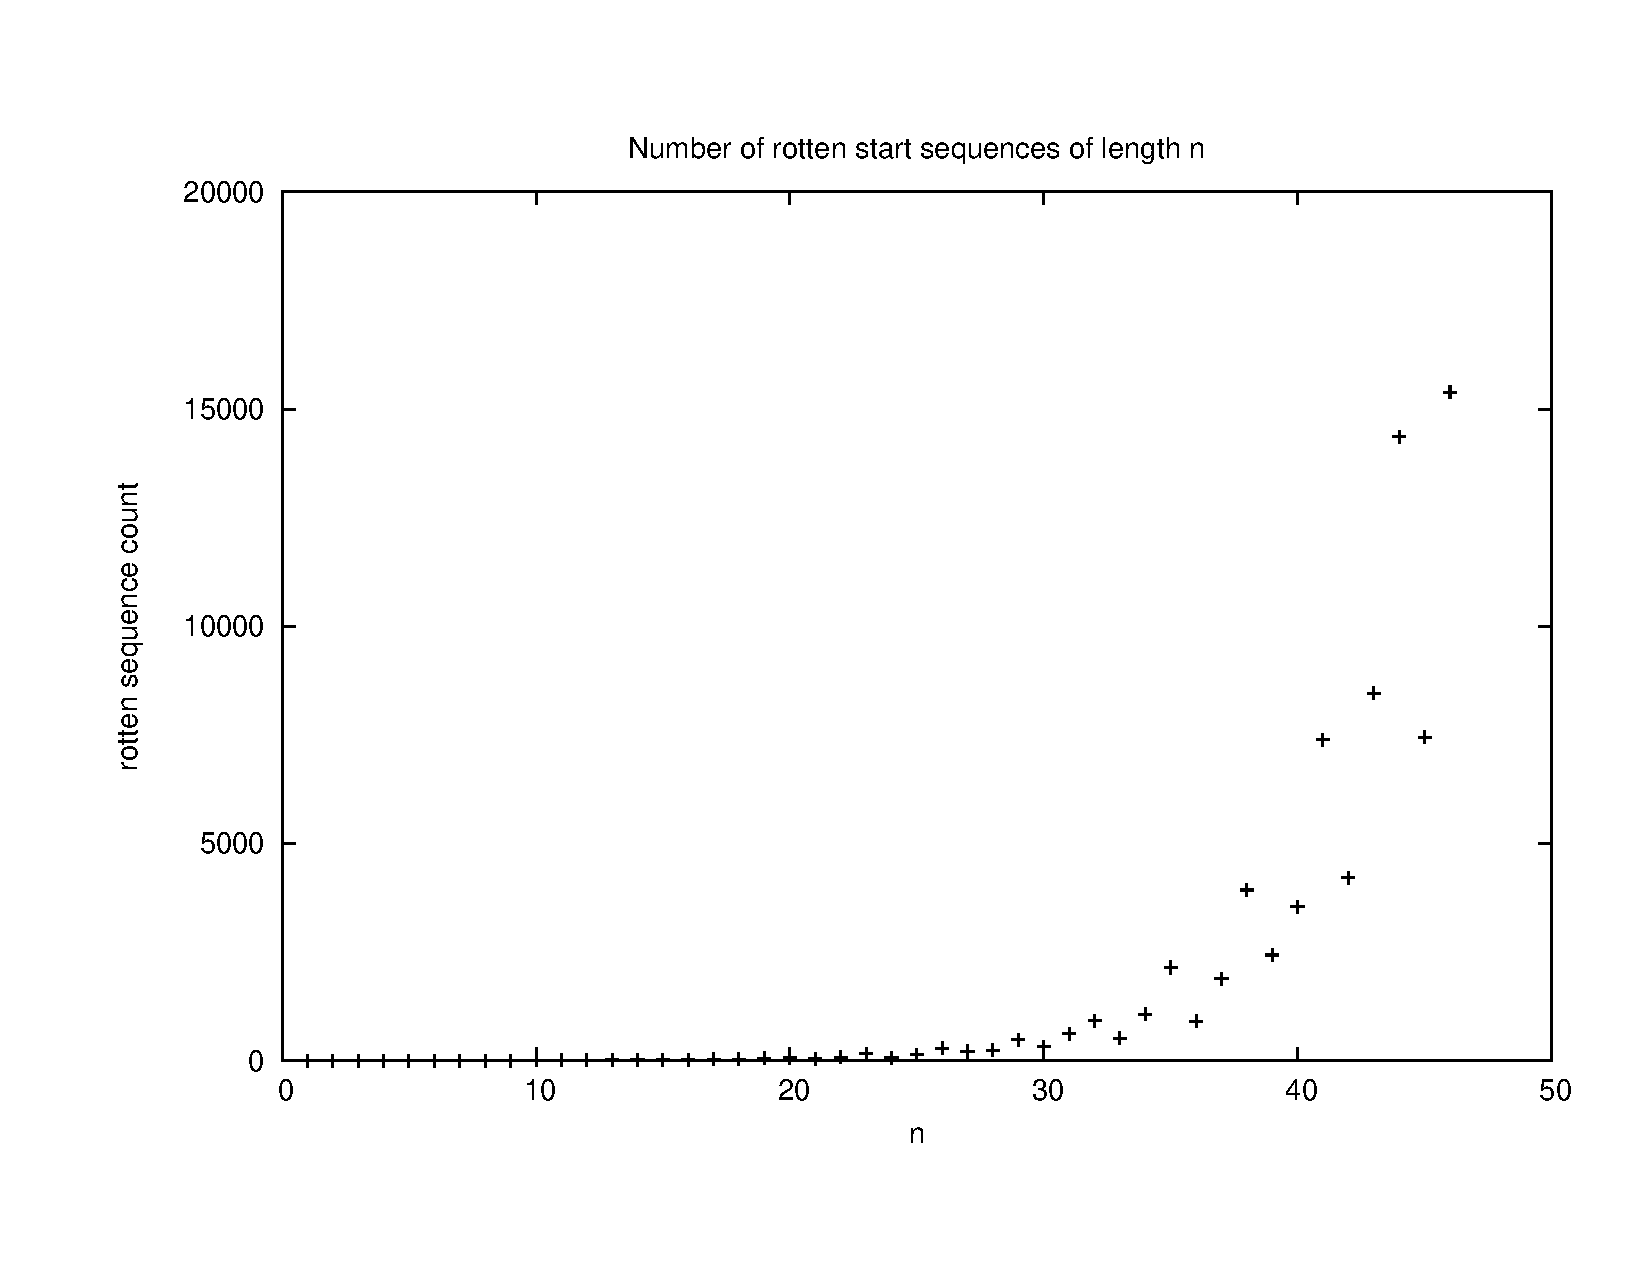
\includegraphics[width=4in]{rotten.pdf}
\end{center}
\caption[]{FIX FOR 48: Graph of counts of rotten sequences, lengths 1 through 47.}
\end{figure}

\begin{table}\label{tab:act}
\begin{center}
\begin{tabular}{rrrrrrrrrr}
?& 1& 2& 1& 5& 3& 12& 9& 19& 16\\
38& 20& 59& 42& 104& 65& 213& 111& 400& 245\\
765& 439& 1563& 820& 3046& 1731& 5955& 3292& 12078& 6343\\
23841& 13090& 47204& 25534& 95140& 50154& 189045& 101861& 376225& 201242\\
\end{tabular}
\end{center}
\caption[]{Number of active sequences of lengths 2 through 40. (A217437)}
\end{table}
\begin{figure}\label{fig:act}
\begin{center}
\includegraphics[width=4in]{active.pdf}
\end{center}
\caption[]{FIX FOR 41+: Graph of counts of active sequences, lengths 1 through 40.}
\end{figure}

\subsection{Computational Details}
Here, a brief discussion of the harmony project.

\section{Results}\label{sect:results}

\section{Conclusions}\label{sect:conclusions}
\section*{Appendix: Proofs}\label{app:proofs}
\ni{\bf Proof of Lemma~\ref{lemma:p4}.} We prove by contradiction.  Assume that for nontrivial, $T$, $T^4$ appears
in the word generated by iteratively rewriting some nonterminal $k$ times, where $k$ is minimal.
Rather obviously, $k>1$, since the expansions of \q{a} and \q{b} do not contain
such a string.  Also note that $T$ must contain a \q{b} symbol since $a^4$ never
occurs.  Indeed, if it contained only one \q{b}, then we would have
 $$T=UbV$$
 $$T^4=UbVUbVUbVUbV$$
\ni but the $b$-free string $VU$ necessarily separates four consecutive \q{b} symbols
by equal distances which, by Observation~\ref{obs:fourb}, cannot happen.  The string $T$ then, must have
two or more \q{b} symbols.

Suppose $T$ contains exactly two $b$'s, and consider the adjacency of $T$'s.
$$\underbrace{P\cdot b\s{x}b\s{y} }_T\underbrace{b\s{x}b\s{y} }_T\underbrace{b\s{x}b\s{y} }_T\underbrace{b\s{x}b\cdot Q}_T$$
\ni where $y=|P|+|Q|$.  Clearly, $x$ and $y$ must differ, lest we violate Observation~\ref{obs:fourb}.  
Suppose $x=1$ (signaling the left of a rewrite of \q{b}), then the spacings are either $1-2-1-2-1$ or
$1-3-1-3-1$, neither of which is possible after a valid rewriting.  A similar argument holds for all other
pairs of assigning values to $x$ and $y$.  $T$, therefore must have three or more $b$'s.

If $T$ contains several $b$'s we can think of the quadruple $T$ as
$$T^4=\underbrace{P\cdot b\s{z}\cdots b\s{x}b\s{y} }_T\underbrace{b\s{z}\cdots
  b\s{x}b\s{y} }_T\underbrace{b\s{z}\cdots b\s{x}b\s{y}
}_T\underbrace{b\s{z}\cdots b\s{x}b\cdot Q}_T$$ \ni where, again, $y=|P|+|Q|$.
Here, Observation~\ref{obs:fourb} suggests that $x$, $y$, and $z$ cannot all
be equal, and one or two must be $3$.  Suppose $x=1$, then $y=z=3$ and we
force $Q$ (and what follows) to be the result of rewriting a \q{b}.  The entire
string $T^4$ must be the result of rewriting $S^4$ where $S=u\cdot B$.  This,
however, is not possible since the appearance of $T^4$ was the first,
minimizing the number of rewrites, $k$.  A symmetric argument leads to a
contradiction when $z=2$.

When $y=1$, $P$ is forced to be a singleton, with $T^4$ preceded by a \q{b}, which is sufficient to make it the image
of $S^4$ where $S=b\cdot U$, which contradicts the first appearance of a quadruple.  When $y=2$, then $Q$ must be a pair with $T^4$ immediately followed by a \q{b} and $T^4$ appears in the result of rewriting four copies of $S=U\cdot b$, leading to a contradiction.

Perhaps the adjacency of $T$'s appears fully between rewriting of $b$'s.  In these cases $x=2$ or $z=1$ or both, with
$y=3$.  Whenever $x=2$, then $Q$ is part of a triple, and $T^4$ appears as the result of rewriting $S^4$ where $S=U\cdot ba$.  Whenever $z=1$, then a symmetric argument forces $S=ab\cdot U$.

Having shown every possibility for $T$ leads to a contradiction, we find the theorem true.\QED

\ni{\bf Proof of Lemma~\ref{lem:propercurl}.}
\Proof Suppose it did.  Then there exists and \abs\ $S=\mu(S')=XY^3aZ$, with $Y$ nonempty.
$S$ must appear in the expansion of \q{a}.  Let's assume this happens, first,
after $k$ rewrites.  (ie. that $S$ is a subword of $\mu^k(a)$ containing this
pattern).   First,
we realize, by inspection, that $k>1$ since no pattern of this form appears
in the rewrite of $\mu(a)=aaba$.

Suppose we have $S=XYYYa\cdots$.  Then $Y$ must contain both an \q{a} and a \q{b},
at least.  It is not difficult to see that $\mu(aUa)$ must contain an equal
number of $bab$ and $baab$ sequences, and that they appear in pairs as
part of the rewriting of each \q{b}: $$\mu(aba)=aa\underbrace{bab}aaabaaa\underbrace{baab}a=aab\s{1}b\s{3}b\s{3}b\s{2}ba$$
\ni Now, if $Y$ is $ab$ (or $ba$), then $Y^3$ has the form $ab\s{1}b\s{1}b$
(or $b\s{1}b\s{1}ba$), whose adjacent singletons are illegal.  Similarly
all rotations of $aab$ for adjacent pairs.  Rotations of $aaab$ are illegal
because they form three adjacent triples, which cannot happen, due to Observation~\ref{obs:fourb}.  It follows, then, that $Y$ must have matching numbers
of single and double $a$'s.  

There are two cases: when the singletons appear to the left of respective doubles---
that is, all expansions of \q{b} appear within $Y$, and when the doubles appear to the left of the singletons---when some expansion of \q{b} crosses the $YY$ boundary.
Suppose $Y=Ub\s{3}b\cdots \s{3}bV$, where $U=\cdots\s{1}$ and $V=\s{2}\cdots$.  Then $V\cdot U$ must be the expansion of $n$ $a$'s: $VU$ is $\mu(a)=aaba$, $\mu(aa)=aabaaaba$, or $\mu(aaa)=aabaaabaaaba$.
Then, with some thought about forced patterns the boundary strings $X$ and $aZ$, we can write $XU=X'\mu(a^r)$ and $VaZ=\mu(a^t)Z'$, where
$r+t=n+1$ and $V$ is at least $aab$:
\begin{align*}
S&=XUb\s{3}b\cdots \s{3}bV\cdot Ub\s{3}b\cdots \s{3}bV\cdot  Ub\s{3}b\cdots \s{3}bV\cdot a\\
 &=X'\mu(a^r)\mu(P)\mu(a^n)\mu(P)\mu(a^n)\mu(P)\mu(a^t)Z'
\end{align*}
\ni where $P$ begins and ends with a \q{b} (or $P=b$) and thus
\begin{align*}
S &=X'\mu((a^rPa^{t-1})^3a)Z'
\end{align*}
\ni which is the rewrite of an \q{a} with a curl of 3, contradicting the minimum selection of $k$.

Otherwise, suppose an expansion of \q{b} spans the $YY$ interface.  Then $Y=U\s{2}b\cdots b\s{1}V$,
where $VU=baaabaaab$.  Then
\begin{align*}
S&=XY^3aZ\\
 &=XU\s{2}b\cdots b\s{1}V\cdot U\s{2}b\cdots b\s{1}V\cdot U\s{2}b\cdots b\s{1}V\cdot aZ
\end{align*}
\ni We set $aPa$ to be the preimage of the sequence $\s{2}b\cdots b\s{1}$ in $Y$. If $U$ is not empty, we have $XU=X'\mu(b)$ and if $V$ is not empty,
we have $VaZ=\mu(ba)Z'$:
\begin{align*}
S &=X'\mu(b)\mu(aP)\mu(b)\mu(P)\mu(b)\mu(P)\mu(ba)Z'
\end{align*}
\ni If $V$ is empty, then $VaZ=aabaZ'=\mu(a)Z'$
\begin{align*}
S &=X'\mu((bP)^3)\cdot \mu(a)Z'
\end{align*}
\ni which is contradictory.

Having considered all the possiblities, the theorem is shown to be true.
\QED

\ni{\bf Proof of Lemma~\ref{lem:abcurl}.} We seek to demonstrate that each $a_i$ is at least 2 and each $b_i$ is 3.
Lemma~\ref{lemma:p4} demonstrates that the maximum number of times any substring
repeats is less than 4.  Likewise for any $a_i$ we need only demonstrate a curl
of 2 since Lemma~\ref{lem:properacurl} eliminates the possiblity that it is greater.

\ni {Case $a_2$.} We note that $b\rightarrow b\cdot a\cdot a\cdot a_2baaab$, thus $a_2$ has curl 2.

\ni{Case $b_1$.}  We note that $b\rightarrow b\cdot a\cdot a\cdot a\cdot b_1aaab$, thus $b_1$ has a curl of 3.

\ni{Case $a_5$.} Similar patterns validate $a_5$ and $b_2$:
\begin{align*}
b&\rightarrow baaab\cdot a \cdot a \cdot a_5b\\
b&\rightarrow baaab\cdot a \cdot a \cdot a\cdot b_2
\end{align*}
\ni demonstrating respective curls of 2 and 3.

\ni Each of these cases is simple, demanding no context beyond the rewrite of a single letter. The validation of the remaining symbols is sensitive to the context of the rewritting of letters in the predecessor.

Let's consider $a_0$.  Here, we make use of the knowledge of symbols forced immediately
to the left of the rewritten \q{b}.  Since every \q{b} is preceded by an \q{a} we have:
\begin{align*}
a\cdot b&\rightarrow a\cdot ab\cdot ab\cdot a_0a_1abaaab
\end{align*}
Similarly, $a_1$ is preceded by $ba$ by ``rotating'' the pattern that
validates $a_0$.

Let's consider $a_6$, which comes from the expansion of an \q{a}. Because
$a_6$ is on the left edge of the expansion, we must develop further leftmost
context.  The \q{a} is preceded by any of $ab$, $aba$, or $abaa$:
\begin{align*}
ab\cdot a&\rightarrow aabab\cdot aaab\cdot aaab\cdot a_6a_7ba\\
aba\cdot a&\rightarrow aababaaabaa\cdot aba \cdot aba\cdot a_6a_7ba\\
abaa\cdot a&\rightarrow aababaaabaaab\cdot aaba\cdot aaba\cdot a_6a_7ba
\end{align*}
\ni Notice that any verification of $a_6$ can be turned into a verification
of the following $a_7$ by dropping the leftmost character (which is always
an \q{a}) and appending the character immediately to the right.  

The proof
of the validity $b_3$ is similar:
\begin{align*}
ab\cdot a&\rightarrow aab\cdot abaa\cdot abaa\cdot abaa\cdot b_3a\\
aba\cdot a&\rightarrow aababaaabaaabaab\cdot a\cdot a\cdot a\cdot b_3a\\
abaa\cdot a&\rightarrow aababaaabaaabaabaaaba\cdot a\cdot a\cdot b_3a
\end{align*}
\ni Finally, the $a_8$ is demonstrated as follows:
\begin{align*}
ab\cdot a&\rightarrow aababaaaba\cdot aab\cdot aab\cdot a_8\\
aba\cdot a&\rightarrow aababa\cdot aabaaab\cdot aabaaab\cdot a_8\\
abaa\cdot a&\rightarrow aababaaabaaabaab\cdot aaab\cdot aaab\cdot a_8
\end{align*}

\ni Case $b_0$. We note $b_0$ occurs in the expansion of a \q{b} preceded
by at most three \q{a} symbols.

\ni If $b_0$ occurs after a triple \q{a}, we have 
$$aaa\cdot b\rightarrow aaba\cdot aaba\cdot aaba\cdot b_0aaabaaab$$

\ni If $b_0$ occurs following a double \q{a}---the marker for the right side
of a \q{b} expansion---we can deduce more context: $abaaabaaab\cdot aab$.
The validation of a curl of 3 is straightforward:
\begin{align*}
abaa\;abaa\;abaa\cdot b\rightarrow&aababaaabaaabaabaaaba\\
&aababaaabaaabaabaaaba\\
&aaba\;baaabaaabaabaaaba\cdot b_0aaabaaab
\end{align*}

\ni In cases where a single \q{a} appears before a \q{b}:
$$bab'_0$$
\ni the image appears as, itself, $bab_0$:
$$baaabaaab~aaba\cdot b_0aaabaaab$$
\ni which does not provide enough context to validate the $b_0$.  Suppose, however, that the $b'_0$ is
proven correct, say by the pattern $TTTb'_0$, as might happen by recursive application of one
of the prior cases.  Then it must be the case that the rewrite is $\mu(T)\mu(T)\mu(T)b_0$ which is sufficient
to demonstate the necessary pattern.  Thus, if the address of $b_0$ ends in the finite string $\cdots xb_0\cdots b_0b_0b_0$ where $x$ is validated, induction demonstrates the validity of each of the $b_0$ instances.  Otherwise,
validation fails.  We term instances of $b_0$ whose heritage suffixes contain only instances of $b_0$ a
\term{left edge}.

Cases $a_3$ and $a_4$. We note that the $a_4$ is validated by the same string, rotated, as the $a_3$.
This results from the fact that the validation of the $a_3$ ends in a \q{b}, so
it must start in a \q{a} (lest the repeat generated adjacent $b$'s).  This means
the repeated sequence can have its initial \q{a} moved to the end, after the
\q{b}, validating the $a_4$.  Thus we only consider the validation of $a_3$.

Any instance of $a_3$ has address \addr{\cdots b_ia_3}, where $i$ is between 0 and 3.  In any instance
where the $b_i$ is prefixed by 2 (or even 3) $a$'s we have
\begin{align*}
 \cdots aa\cdot b_i&\rightarrow a\cdot abaaab\cdot abaaab\cdot a_3aab
\end{align*}

The only situation where $b_i$ is prefixed by a single \q{a} is, as we have
seen, when $i=0$, where the addresses end \addr{\cdots b_jb_0a_3}.  Notice that the
string immediately to the left of $a_3$ is always $baaab$.  This, in turn is
always preceded by an expansion of the left context of $b_j$ which is always
an \q{a}:
$$aaba\;aaba\;baaabaaab\;aaba\cdot baaaba_3$$ Suppose that $j$ is $2$, that is
that the $a_3$ is in the expansion of a right-most \q{b} in a \q{b} re-write.
Then we have a 141 character repeat:
\begin{align*}
baaabaaa\cdot b_2\rightarrow{} & baaabaaab~aaba~aaba~aaba~baaabaaab~aaba~aaba~aaba\cdot b_0aaabaaab\\
\rightarrow baaab\cdot{}aaab&\s{2}b\s{3}b\s{3}b\s{1}b\s{3}b\s{3}b\s{2}b\s{3}b\s{3}b\s{1}b\s{3}b\s{3}b\s{2}b\s{3}b\s{1}b\s{3}b\s{3}b\s{2}b\s{3}b\s{3}b\s{1}b\s{3}b\s{3}b\s{2}b\s{3}b\s{3}b\s{1}b\s{3}b\s{3}b\s{2}b\s{1}baaab\cdot\\
  aaab&\s{2}b\s{3}b\s{3}b\s{1}b\s{3}b\s{3}b\s{2}b\s{3}b\s{3}b\s{1}b\s{3}b\s{3}b\s{2}b\s{3}b\s{1}b\s{3}b\s{3}b\s{2}b\s{3}b\s{3}b\s{1}b\s{3}b\s{3}b\s{2}b\s{3}b\s{3}b\s{1}b\s{3}b\s{3}b\s{2}b\s{1}baaab\cdot a_3\cdots
\end{align*}
\ni This repeat begins with the right portion of \q{b} (5
characters in) in the corresponding $b_1$, followed by the $a_3a_4a_5$ and the
5 characters to the left of the $a_3$.  This is preceded in the span between
$b_0$ and $b_1$.

In cases where the address of $a_3$ does not contain a $b_2$ in any finite
suffix of its address, the curl is insufficint, and is calculated as 1.
\QED

\ni{\bf Proof of Lemma~\ref{lem:abcurl}.} \ni[Ed. This proof to be moved to appendix, or dropped if obvious. \Proof Proof of complementary grammar.  Suppose we label
$$\rmu(a)=a_8b_3a_7a_6$$
\ni then, we have the following cases:

\ni Cases $a_2$, $b_1$, and $a_5$.  Trivially the same.

\ni Case $a_0$.  $b$ is preceded by $a$.  Thus
\begin{align*}
aba\cdot b&\rightarrow abaabaaabaaababaaba_0aabaaab FIX\\
abaa\cdot b&\rightarrow abaabaaabaaababa\cdot aab\cdot aab\cdot a_0aabaaab\\
abaaa\cdot b&\rightarrow abaabaaabaaababaaaba\cdot aab\cdot aab\cdot a_0aabaaab
\end{align*}

\ni Case $a_7$. We're expanding the letter \q{a}:
\begin{align*}
ab\cdot a&\rightarrow abaabaaabaa\cdot ab\cdot ab\cdot a_7a\\
aba\cdot a&\rightarrow abaabaa\cdot abaaab\cdot abaaab\cdot a_7a\\
abaa\cdot a&\rightarrow abaabaaabaaabab\cdot aaab\cdot aaab\cdot a_7a
\end{align*}

\ni Case $a_6$. We're expanding the letter \q{a}:
\begin{align*}
ab\cdot a&\rightarrow abaabaaabaaa\cdot ba\cdot ba \cdot a_6\\
aba\cdot a&\rightarrow abaabaaa\cdot baaaba\cdot baaaba \cdot a_6\\
abaa\cdot a&\rightarrow abaabaaabaaababa\cdot aaba\cdot aaba\cdot a_6
\end{align*}

\ni Case $a_8$. We're expanding the letter \q{a}:
\begin{align*}
ab\cdot a&\rightarrow abaab\cdot aaab\cdot aaab\cdot a_8baa\\
aba\cdot a&\rightarrow abaabaaabaaabab\cdot a\cdot a\cdot a_8baa\\
abaa\cdot a&\rightarrow abaabaaabaaababaaab\cdot a\cdot a\cdot a_8baa
\end{align*}

\ni Case $b_3$. We're expanding the letter \q{a}:
\begin{align*}
ab\cdot a&\rightarrow ab\cdot aaba\cdot aaba\cdot aaba\cdot b_3aa\\
aba\cdot a&\rightarrow abaabaaabaaabab\cdot a\cdot a\cdot a\cdot b_3aa\\
abaa\cdot a&\rightarrow abaabaaabaaababaaab\cdot a\cdot a\cdot a\cdot b_3aa
\end{align*}
FINISH
\QED]

\ni{\bf Proof of Theorem~\ref{thm:aperiodic}.} (motivated by Gr\"unbaum, p. 573, 10.6.3).
An infinite \ab-sequence (a \term{curly sequence}) cannot be written as infinitely many repetitions of
a finite block of $a$'s and $b$'s.

Suppose it were the case—--that is an infinite \ab-sequence $\scS$ can be
written as a finite sequence $S$ of length $m$, repeated.  Then, since $\scS$
is an curly sequence its terms can be composed consistently using the
\abg, forming a precursor sequence, $\scS'$ (which is also curly) with
each letter of $\scS^{-1}$ expanding to 4 (in the case of an \q{a}) or 9 (in the
case of a \q{b}) letters in $\scS$.  We may, of course do this any finite number
of times, say, $n$, yielding $\scS^{-n}$ whose letters that span more than
$4^n$ letters in $\scS$.  If $n$ is sufficiently large, then $m < 4^n$.  But
shifting by $m$---a supposed symmetry of $\scS$ does not yield a symmetry in
$\scS^{-n}$, so we have that $\scS$ is non-periodic.\QED

\ni{\bf Alternative proof.}(Modeled after Senechal\cite{Se95})  
We remind the reader that the
rewriting matrix for the \abg\ is \term{primitive}.  A primitive matrix
\q{Q} is one whose entries are non-negative with, for some $k$, the entries of
$Q^k$ are all positive. (For our rewriting grammar, $k=1$.)  Such a matrix
demonstrates that ``all letters eventually appear'' in the rewriting of any
patch of letters.  It is sufficient, then to consider the rewriting of the
letter \q{a}.  Here, $a\rightarrow aaba \rightarrow aababaaabaaab \rightarrow \cdots$.  At each stage we can count the number of letters that
appear, and we can compute the ratio of $a$'s and $b$'s.  As we demonstrated
in the text the ratio of $a$'s to $b$'s is $\sqrt{6}$ to $1$.  Since
$\sqrt{6}$ is irrational the rewriting system does not generate an infinite
periodic sequence.  Why? If the sequence had been periodic, there would be
rational ratio of $a$'s and $b$'s in each block, preserved through simple
repetition.\QED

\medskip
\ni(Local Isomorphism.)  Here, we seek to prove that every finite subsequence, $S$, of letters of a curly sequence appears in infinitely often elsewhere in the sequence.

Here, we again note that every infinite curly sequence is the result of
rewriting a precursor sequence $\scS^{-1}$, itself infinite and curly.
Considering precursors some finite number of steps---say $n$---back, we can encapsulate
the finite subsequence in the image a single letter.  All letters, of course,
appear infinitely often, so in their images the finite subsequence must also
appear infinitely often.  Furthermore, it is possible to identify a bound
on $n$ as a function of the diameter of the patch.  This, along with the fact
that no letter is farther than 4 from an equivalent identifies an upperbound
on the distance that must be traveled in $\scS$ to find a patch congruent with
$S$.  We have, then, demonstrated the Local Isomorphism property.\QED

\newpage
\pagestyle{empty}
\nocite{Ch09,Ch13,VDB07}
\bibliographystyle{plain}
\bibliography{references}
\end{document}

Thoughts on property P2.

Suppose we have an especially good starting sequence, S.  Then S begins
with a 2.

Proof:
  Suppose, instead, that it began with a 3.  This 3 is not neutral because
if it was neutral, then we could remove the 3 and the shorter sequence would
have a tail, just as long, contradicting the fact that this is the first
sequence that has a tail so long.
  Since the 3 is not neutral, it is the beginning of a Y that supports a
curling number, c, at some point in the tail, lc+1, where |Y|=l.  
Of course, c could be 2 or three.
  Suppose it is 2.  Then we have this diagram
  3...3...2... = SS(e)
  Y-->Y-->2...
  ^   ^   ^
  1   l+1 2l+1


  Suppose c=3.  Then we have this diagram
  3...3...3...3... = SS(e)
  Y-->Y-->Y-->3...
  ^   ^   ^   \
  1   l+1 2l+1 3l+1
Now let Y' be Y with the leftmost 3 rotated to be rightmost
(e.g. Y=323222 becomes Y'=232223) then we know SS(e) begins
  3Y'Y'Y'...
which means that the curl at 3l+2 is 3, which places 2 3's in a row which
(besides violating proposed property P3) terminates the sequence.
[Why this might be bad: the position 3l+1 seems quite early for a long tail to end.]

[Corollary: the Y that proves a curl of 3 does not start with 3.]

